\section{SYCL未来发展方向}
现在请花点时间感受一下平和与平静,因为我们已经介绍了使用 C++ 和 SYCL 进行编程。 所有的部分都已就位。

我们努力确保前几章中的代码示例使用标准 SYCL 2020 功能并在各种硬件上执行,
并且我们在少数地方使用了扩展(例如互操作性和 FPGA 特定扩展),我们将其指出。 
然而,截至 2023 年中期,本尾声中显示的面向未来的代码无法使用任何编译器进行编译。

在这篇尾声中,我们推测未来。 我们的水晶球可能有点难以阅读——这个尾声没有任何保证。 
我们在本书第一版中做出的一些预测实现了,但其他预测却没有实现。

本尾声让我们先睹为快,了解即将推出的 SYCL 功能和 DPC++ 扩展,我们对此感到非常兴奋。 
我们不保证本尾声中打印的代码示例可以编译:有些可能已经与本书之后发布的编译器兼容,
而另一些则可能仅在一些语法调整后才能编译。 
某些功能可能会作为扩展发布或合并到 SYCL 的未来版本中,而其他功能可能会无限期地保留为实验性功能。 
与本书相关的 GitHub 存储库中的代码示例可能会随着其发展而更新以使用新语法。 
同样,我们也会对本书进行勘误,并且可能会不时进行补充。 
我们建议检查这两个地方的更新(代码存储库和书籍勘误表 - 链接可以在第 1 章前面找到)。

\subsection{与 C++11、C++14 和 C++17 更紧密地结合}
保持 SYCL 和 C++ 之间的紧密一致有两个优点。 
首先,它使 SYCL 能够利用 C++ 的最新、最强大的功能来提高开发人员的工作效率。 
其次,它增加了 SYCL 中引入的异构编程功能成功影响 C++ 未来方向的机会。

SYCL 1.2.1 基于 C++11,SYCL 2020 接口的许多最大改进只能通过 C++14(例如通用 lambda)
和 C++17(例如 ,类模板参数推导——CTAD)。 
我们预计 SYCL 和 C++ 随着时间的推移会变得越来越接近,并且已经有一些令人兴奋的工作正在进行中。

C++ 标准模板库 (STL) 包含几种与第 17 章中讨论的并行模式相对应的算法。
STL 中的算法通常适用于由迭代器对指定的序列,并且从 C++17 开始支持执行策略参数 表示它们应该顺序执行还是并行执行。 
该标准还允许实现定义自己的执行策略,
第 18 章中介绍的 oneAPI DPC++ 库 (oneDPL) 利用此类自定义执行策略来使算法能够在 SYCL 设备上执行。 
其结果是一种高生产率的异构设备编程方法 - 如果可以仅使用 STL 算法的功能来表达应用程序,
oneDPL 就可以在我们的系统中使用加速器,而无需编写一行 SYCL Kernel代码! 
关于 STL 算法应如何与某些 SYCL 概念(例如缓冲区)交互,
以及如何确保我们可能需要的所有标准库类(例如 std::complex、std::atomic)可用,
仍然存在悬而未决的问题 在设备代码中,但 oneDPL 是统一主机和设备代码的漫长道路上的第一步。

\subsection{采用 C++20、C++23 及其他版本的功能}
SYCL 规范故意落后于 C++,以确保它使用的功能具有广泛的编译器支持。 
然而,SYCL 委员会成员(其中许多人还参与了 ISO C++ 委员会)正在密切关注 C++ 未来版本的开发情况。

采用我们在此讨论的尚未最终确定为规范的 C++ 或 SYCL 功能可能会是一个错误——功能在成为标准之前可能会发生重大变化。 
尽管如此,有许多正在讨论的功能可能会改变未来 SYCL 程序的外观和行为方式,值得讨论。

SYCL 2020 中的一些功能由 C++20 通知(例如 std::atomic\_ref),
其他功能则预先采用到 sycl:: 命名空间中(例如 std::bit\_cast、std::span)。 
当我们迈向 SYCL 的下一个正式版本时,我们希望与 C++20 更加紧密地保持一致,并合并其中最有用的部分。 
例如,C++20以std::latch和std::barrier的形式引入了一些额外的线程同步例程; 
我们已经在第 19 章中探讨了如何使用类似的接口来定义设备范围的屏障,
并且在新的 C++20 语法的上下文中重新检查子组和工作组屏障也可能有意义。

C++23 中最令人兴奋的功能之一是 mdspan,它是一种非拥有数据视图,
它提供指针的多维数组语法和 AccessorPolicy 作为控制对底层数据的访问的扩展点。 
这些语义与 SYCL 访问器的语义非常相似,
并且 mdspan 将使类似访问器的语法能够用于缓冲区和 USM 分配,如图 EP-1 所示。

\begin{figure}[H]
	\centering
	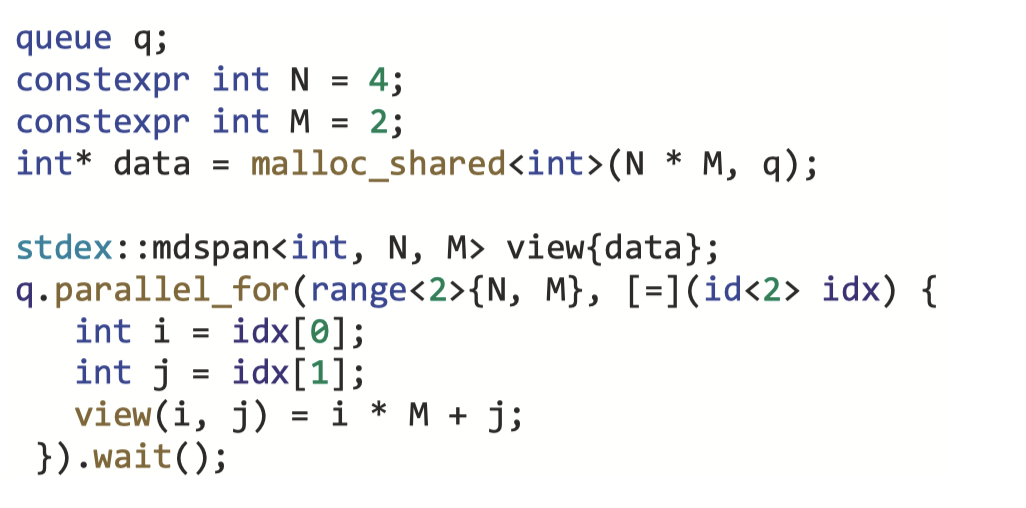
\includegraphics[width=0.9\textwidth]{figs/F22.1.png}
	\caption{\textit{使用 mdspan 将类似访问器的索引附加到 USM 指针 }}
\end{figure}

希望 SYCL 正式支持 mdspan 只是时间问题。 
同时,我们建议感兴趣的读者尝试作为 Kokkos 项目一部分提供的开源生产质量参考实现。

\subsection{混合 SPMD 和 SIMD 编程}
C++ 的另一个令人兴奋的提议功能是 std::simd 类模板,它旨在为 C++ 中的显式向量并行性提供可移植接口。 
采用此接口将明确区分第 11 章中描述的向量类型的两种不同用途:为了程序员的方便而使用向量类型,
以及忍者程序员为了低级性能调整而使用向量类型。 
同一语言中对 SPMD 和 SIMD 编程风格的支持也引发了一些有趣的问题:我们应该如何声明Kernel使用哪种风格,
以及我们是否应该能够在同一Kernel中混合和匹配风格?

我们已经开始以 DPC++ 扩展 (sycl\_ext\_oneapi\_invoke\_simd) 的形式探索这个问题的潜在答案,
它提供了一个新的 invoke\_simd 函数(在 std::invoke 上建模),
允许开发人员从 SPMD 中调用显式矢量化 (SIMD) 代码 核心。 
对invoke\_simd 的调用充当两种编程风格所隐含的两种执行模型之间的清晰边界,并定义数据应如何在它们之间流动。 
图 EP-2 中的代码显示了 invoke\_simd 用法的一个非常简单的示例,调用一个期望接收标量和向量 (simd) 参数组合的函数。

\begin{figure}[H]
	\centering
	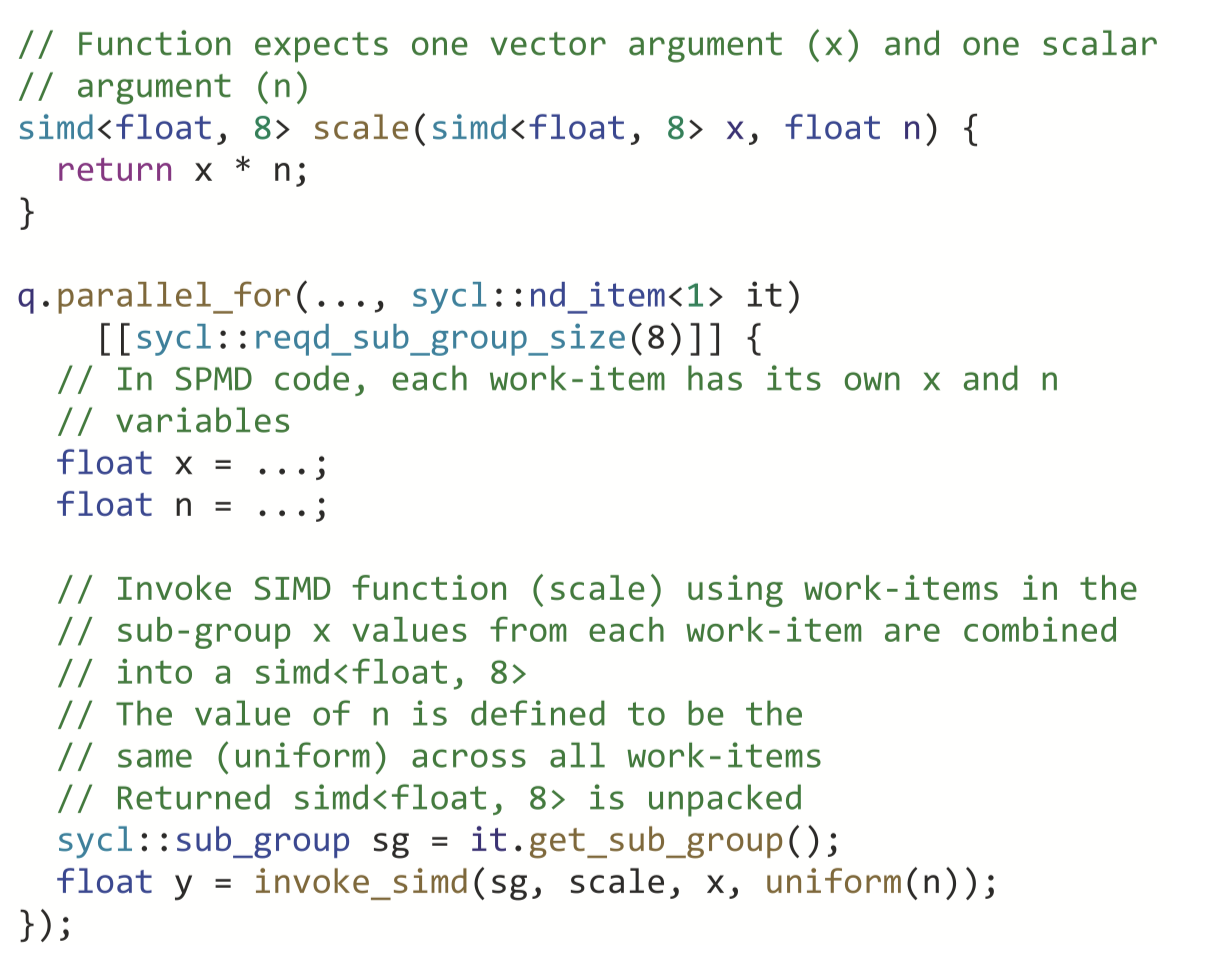
\includegraphics[width=0.9\textwidth]{figs/F22.2.png}
	\caption{\textit{从 SPMD Kernel调用 SIMD 函数的简单示例 }}
\end{figure}

invoke\_simd 采用的方法有几个优点。 首先,不会出现令人讨厌的意外——显式调用具有不同执行模型的函数,
并且用户负责描述如何来回编组数据。 
其次,该机制允许细粒度的专业化——可以只编写几行显式矢量化代码(例如,用于性能调整),而不必丢弃其余的 SPMD 代码。 
最后,扩展很简单——invoke\_simd 本身可以通过简单的重载来扩展以支持新组或新参数映射,
并且可以引入类似的 invoke\_* 函数来处理与不同上下文的互操作性(例如,用非 SYCL 语言编写的代码)。

\subsection{地址空间}
SYCL 2020 中引入的通用地址空间支持有可能极大地简化许多代码,因为它允许我们使用常规 C++ 指针,
而不必担心正在使用哪种内存。 许多现代体系结构为通用地址空间提供硬件支持,
因此我们可以期望使用常规 C++ 指针的代码能够在各种机器上工作,并且性能开销最小。

然而,在某些(较旧的或更特殊用途的)体系结构上,通用地址空间支持是一个更复杂的故事。 
一些硬件可能使用不同的指令来访问不同类型的内存,要求编译器在编译时识别具体的地址空间(即生成正确的指令)。 
还可能存在无法表示通用地址空间的 SYCL 后端(例如 OpenCL 1.2)。 
SYCL 2020 通过一组用于推导地址空间的推理规则来允许此类硬件和后端。

地址空间推导规则继承自 SYCL 1.2.1,SYCL 2020 规范包含一条注释,表明将在 SYCL 的未来版本中重新审视这些规则。 
尽管在撰写本文时尚不清楚这些规则将如何改变,
但 SYCL 的长期想法是明确的:在大多数情况下,我们不应该关心地址空间管理,而应该相信编译器和硬件会做正确的事情。

\subsection{特化机制}
计划引入编译时查询,使Kernel能够根据目标设备的属性(方面)进行专门化
(例如,设备类型、对特定扩展的支持、工作组本地内存的大小、子组) 大小由编译器选择)。 
此类查询需要一种当前在 C++ 中不存在的新型常量表达式,
它们在编译主机代码时不一定是 constexpr,但在目标设备已知时变为 constexpr。

用于公开这种“设备常量表达式”概念的确切机制仍在设计中。 
我们希望它建立在 SYCL 2020 中引入的专门化常量功能的基础上,并且外观和行为与图 EP-3 中所示的代码类似。

\begin{figure}[H]
	\centering
	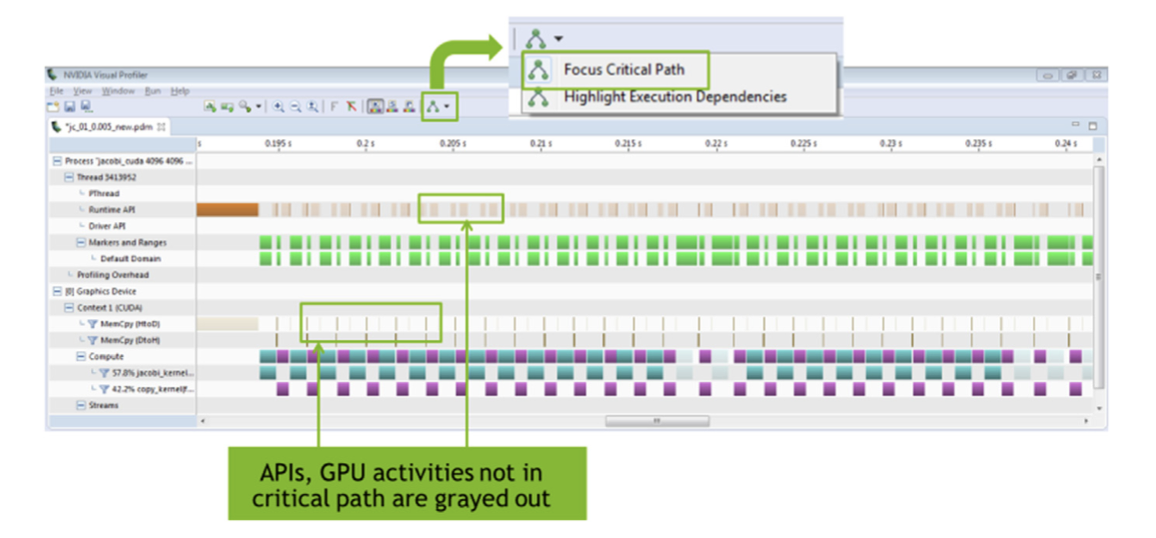
\includegraphics[width=0.9\textwidth]{figs/F22.3.png}
	\caption{\textit{在Kernel编译时根据设备方面专门处理Kernel代码 }}
\end{figure}

\subsection{编译时属性}
SYCL 允许通过将属性列表传递到构造函数来修改某些类(例如缓冲区、访问器)的行为。 
这些属性已经非常强大,但它们的功能受到以下事实的限制:传递给构造函数的属性直到运行时才知道。 
允许在编译时声明某些属性有可能显着提高性能,方法是减少运行时检查的数量,
并使编译器能够在存在特定属性的情况下积极专门化主机和设备代码。

DPC++ 编译器支持编译时属性的实验性扩展 (sycl\_ext\_oneapi\_properties),并且它已经启用了各种其他扩展:

\begin{itemize}
	\item 使用超出地址空间范围的信息注释的指针,
	这可以为 sycl::multi\_ptr 的未来提供信息 (sycl\_ext\_oneapi\_annotated\_ptr)

	\item Kernel配置控制,可以替代 C++ 属性并增强仅库 SYCL 实现的功能 (sycl\_ext\_oneapi\_kernel\_properties)

	\item 所需内存行为和访问控制的描述(sycl\_ext\_oneapi\_device\_global、sycl\_ext\_oneapi\_prefetch)
\end{itemize}

我们在编译时属性方面的早期经验非常积极,并且我们一直在寻找越来越多的潜在用例。 
鉴于其广泛的适用性,我们渴望看到未来 SYCL 规范中采用某些版本的编译时属性。

\subsection{总结}
SYCL 周围已经充满了兴奋,而这仅仅是开始! 我们(作为一个社区)还有很长的路要走,
需要持续不断的努力来提炼异构编程的最佳实践,并设计新的语言功能,以在性能、可移植性和生产力之间达到所需的平衡。

我们需要你的帮助! 如果 SYCL 中缺少您最喜欢的 C++(或任何其他编程语言)功能,请联系我们。 
我们可以共同塑造 SYCL 和 C++ 的未来方向。

\subsection{更多信息}
• Khronos SYCL Registry, www.khronos.org/ registry/SYCL

• H. Carter Edwards et al., “mdspan: A Non-Owning Multidimensional Array Reference,” wg21.link/p0009

• D. Hollman et al., “Production-Quality mdspan Implementation,” github.com/kokkos/mdspan

• Intel DPC++ Compiler Extensions, tinyurl.com/ syclextend